\part{Boolean Tensor Networks}\label{sec:btn}
\section{Introduction}


Now we will explain part of a tool set and framework largely following \cite{CTNS, BB11}.  \marginnote{{\it ``It is not of the essence of mathematics to be conversant with the ideas of number and quantity.''} --- George Boole} Hence, we will approach tensor networks by focusing on familiar components, namely Boolean logic gates (and
multi-valued logic gates in the case of qudits), applied to the tensor network context. See Appendix \ref{sec:Boolean} for background on Boolean algebra.  The concept of Boolean linearity and non-linearity was used to form a dichotomy between fundamental Boolean tensor building blocks in \cite{CTNS}. 

This subject has an increasingly long history.  The first categorical model of Boolean circuits (as well as some progress on the quantum case) can be found in the seminal work by Lafont~\cite{boolean03}.  In the condensed matter community, Boolean tensors, such as \COPY{}-tensors, are very commonly used.  Closely related to Boolean tensors are stabilizer tensors (\S~\ref{sec:stabtt}), sometimes called Clifford tensor networks.  The so called ZX-calculus \cite{CD, Coecke2017} is also built using many Boolean tensors.  

Recall Remark \ref{remark:boolean}.  

\begin{remark}[Terminology: Boolean tensor networks]\label{remark:boolean2}
As previously mentioned in Remark \ref{remark:boolean}.  While in wide use today, the term ``Boolean tensor network'' is not.  We adopt this terminology in our effort to relate tensors with Boolean entries to classical logic gates and networks.  
\end{remark}



\section{Overview of the Chapter}\label{sec:overview}

\subsection*{Tensor network representations of quantum states}\label{sec:newrep}

A qudit is a $d$-level generalization of a qubit.\mn{A q-dit generalization of the quantum circuits and the ZX-calculus appears in \cite{BB11}.  The ZX-calculus is equivalent to Clifford circuits plus cups and caps to bend wires and compose states. It was first proposed in terms of interacting quantum observables in \cite{redgreen}.}  As has been seen in the last section, a quantum state of $n$-qudits has an exact representation as a order-$n$ tensor with each of the open legs corresponding to a physical degree of freedom, such
as a spin with $(d-1)/2$ energy levels. Such a representation, shown in
Figure~\ref{fig:tensor-networks}(a) is manifestly inefficient since it will have a
number of complex components which grows exponentially with $n$. The purpose of
tensor network states is to decompose this type of structureless order-$n$ tensor into
a network of tensors whose order is bounded. \mn{Lafont appears to be the first to work towards a categorical model of quantum circuits~\cite{boolean03}. Many advancements have subsequently been made \cite{CD, redgreen, CTNS, BB11}.} 


There are now a number of ways to
describe strongly-correlated quantum lattice systems as 
tensor-networks. These include
\begin{itemize}
 \item[(i)] Matrix Product States, MPS~\cite{ostromm1995,fannesnachtwern1992,2010NJPh...12b5005C}
 \item[(ii)] Projected Entangled Pair States, PEPS~\cite{verstraete08,TNSreview09}
 \item[(iii)] Multiscale Entanglement Renormalisation Ansatz, MERA~\cite{vidal2007, 2009arXiv0912.1651V}
 \item[(iv)] Tree Tensor Networks, TNN~\cite{PhysRevA.74.022320,2009PhRvB..80w5127T}. 
\end{itemize}

 The central problem faced by all types of tensor networks is that the
resulting tensor network for the quantity $\bra{\psi}(\2 O\ket{\psi}$, where $\2O$
is some product operator, needs to be efficiently contractible (efficient is taken to mean polynomial in the problem size) if any physically meaningful calculations, e.g., expectation values, correlations or probabilities, are to be
computed. For MPS and TTN efficient contractibility follows from the 1D chain or tree-like geometry, while for MERA it follows from its interesting causal cone structure~\cite{2009arXiv0912.1651V}. For PEPS and BTNS, however, exact contraction is not proven to be efficient in general, but can often be rendered efficient if approximations are made~\cite{verstraete08,TNSreview09}.


For MPS and PEPS, shown in Figures~\ref{fig:tensor-networks}(b) and (c), the resulting network of tensors follows the geometry of the underlying physical system, e.g., a 1D chain and 2D grid, respectively. 

Alternatively a Tensor Tree Network (TTN) can be
employed which has a hierarchical structure where only the bottom layer has open physical legs, as shown in Figure~\ref{fig:tensor-networks}(d) 
for a 1D system and Figure~\ref{fig:tensor-networks}(e) for a 2D one.

For MERA the network is similar
to a TTN, as seen in Figure~\ref{fig:tensor-networks}(f) for 1D, but is instead comprised of alternating layers of order-four unitary and order-three isometric
tensors. 

We focus also on tensor with binary entries over $\{0,1\}$.  We use the terminology Boolean tensor network state (BTNS) which is largely unique to this book (see Remarks \ref{remark:boolean} and \ref{remark:boolean2}). We use the terminology to mean a tensor network that contains some algebraically constrained 
tensors obeying some clearly defined diagrammatic laws arising from Boolean logic gates.  Certain widely used classes of tensor network states can be readily exposed
as examples of BTNS \cite{CTNS}.
Specifically, variants of PEPS have been proposed called
string-bond states~\cite{PhysRevLett.100.040501}.  Although these string-bond states, like PEPS in general, are not efficiently contractible, they are efficient to sample. 


\begin{myfullpage}
\begin{illexample}
\label{fig:tensor-networks}

\begin{center}
     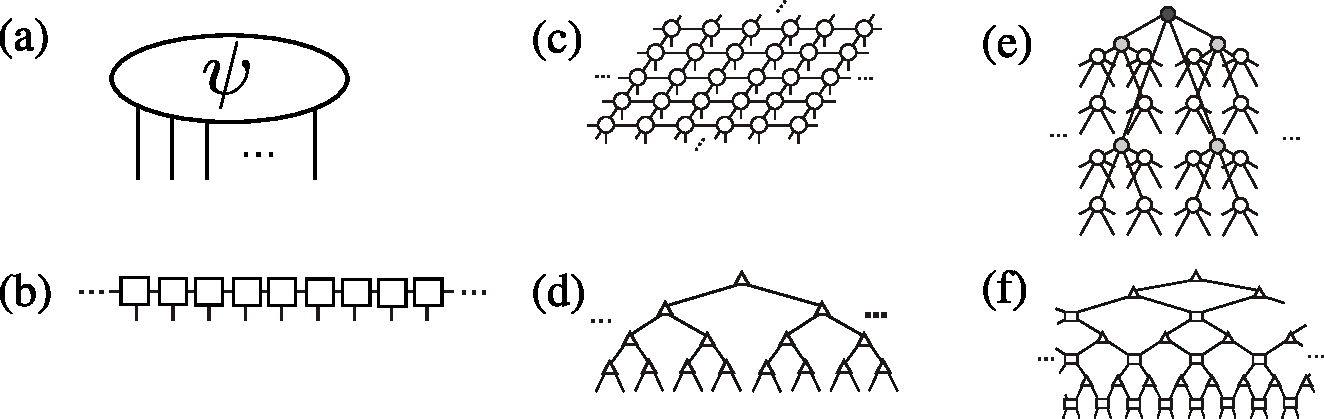
\includegraphics[width=.95\textwidth]{mps_peps_ttn_mera}
\end{center}
(a) A generic quantum state $\ket{\psi}$ for $n$ degrees of freedom represented as a tensor with $n$ open legs. (b) A comb-like MPS tensor network for a 1D chain system~\cite{ostromm1995,fannesnachtwern1992}. (c) A grid-like PEPS tensor network for a 2D lattice system~\cite{verstraete08,TNSreview09}. (d) A TTN for a 1D
chain system where only the bottom layer of tensors possess open physical legs~\cite{PhysRevA.74.022320,2009PhRvB..80w5127T}. (e) A TTN for a 2D lattice system. (f) A hierarchically structured MERA network for a 1D chain system possessing unitaries (order-4 tensors) and isometries (order-3 tensors)~\cite{vidal2007, 2009arXiv0912.1651V}. This tensor network can also be generalized to a 2D lattice (not shown).
\end{illexample} 
\end{myfullpage}

\begin{remark}[Generalisation of String Bond States]
 When recast, certain widely used classes of tensor network states can be readily exposed
as examples of BTNS. Specifically, variants of PEPS have been proposed called
string-bond states~\cite{PhysRevLett.100.040501}.  Although these string-bond states,
like PEPS in general, are not efficiently contractible, they are efficient to sample. By this we mean that for
these special cases of PEPS, any given amplitude of the resulting state (for a fixed computational basis state) can be extracted exactly and efficiently,
in contrast to generic PEPS. This permits variational quantum Monte-Carlo calculations to be performed on string-bond states 
where the energy of the state is stochastically
minimized~\cite{PhysRevLett.100.040501}. This remarkable property
follows directly from the use of a tensor, 
called the {\sf COPY}-tensor, which forms one of several tensors in the fixed
toolbox considered in great detail later in this lecture. 

As its name suggests, the {\sf COPY}-tensor
duplicates inputs states in the computational basis, and thus with these inputs
breaks up into disconnected components, as depicted in
Figure~\ref{fig:stringbonds}(a). By using the
{\sf COPY}-tensor as the ``glue" for connecting up a TNS, the ability to sample the
state efficiently is guaranteed so long as the individual parts connected are themselves
contractible. The generality and applicability of this trick can be seen by examining
the structure of string-bond states, as well as other types of 
similar states like entangled-plaquette-states~\cite{2009NJPh...11h3026M} and
correlator-product states~\cite{2009PhRvB..80x5116C}, shown in Figure~\ref{fig:stringbonds}(c)-(e).  
A long-term aim of this work is that by presenting our toolbox of
tensors, entirely new classes of BTNS with similarly desirable contractibility
properties can be devised. 
\end{remark}
%%%%%%%%%%%%%%%%%%%%%%%%%%%%%%%%%
\begin{myfullpage}
\begin{illexample}
\begin{center}
%\centering
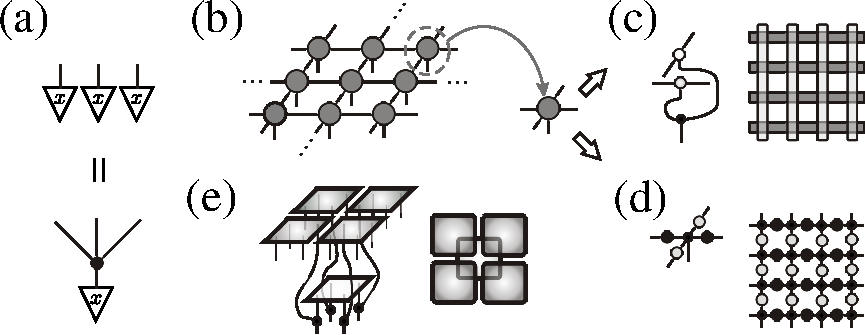
\includegraphics[width=17\xxxscale]{peps_copy_dot}
\end{center}
%\caption{
(a) One of the simplest tensors, the {\sf COPY}-gate or the {\sf COPY}-dot in classical boolean circuits, copies computational basis
states
$\ket{x}$ where $x=0,1$ for qubits and $x=0,1,...,d-1$
for qudits.  The tensor subsequently breaks up into disconnected states.
(b) A generic PEPS in which we expose a single generic order-5 tensor. This
tensor network can neither be contracted nor sampled exactly and efficiently.
However,
if the tensor has internal structure exploiting the {\sf COPY}-tensor, then efficient
sampling
becomes possible. (c) The tensor breaks up into a vertical and a horizontal order-3
tensor joined by the {\sf COPY}-tensor. Upon sampling computational basis states the
resulting contraction reduces to many isolated MPS, each of which are exactly
contractible, for
each row and column of the lattice. This type of state is known as a string-bond
state and can be readily generalized~\cite{PhysRevLett.100.040501}. (d) An even
simpler case is to break the tensor
up into four order-2 tensors joined by a {\sf COPY}-tensor forming a co-called
correlator-product state~\cite{2009PhRvB..80x5116C}. (e) Finally, outside the PEPS
class, there are entangled
plaquette states~\cite{2009NJPh...11h3026M} which join up overlapping tensors (in
this case order-4 ones
describing a $2\times 2$ plaquette) for each plaquette. Efficient sampling is again
possible due to the {\sf COPY}-tensor.\label{fig:stringbonds}
%\end{figure}
\end{illexample}
\end{myfullpage}
%%%%%%%%%%%%%%%%%%%%%%%%%%%%%%%%


\begin{remark}[From qubits, to qtrits, ..., qdits]
 By invoking known theorems asserting the universality of multi-valued logic~\cite{MVL1} (also called $d$-state switching), our methods can be readily applied to tensors of any finite dimension. This was considered explicitly in \cite{BB11}, where a higher dimensional graphical calculus was developed. 
\end{remark}


\subsection*{Tensor network components defined by diagrammatic laws}\label{sec:comdef}

Here we will review the collection of tensors that form a universal
tensor tool box.
In mathematical logic and computer science, formal semantics is an important field of study.  Throughout this lecture series, we largely adopt the semantics 
developed in \cite{CTNS, BB11} which offer a natural extension of the graphical language of quantum circuits in wide spread use in quantum physics.  This was done by merging the overlapping concepts in various fields into a common language that deviates as little as possible from the standard language of quantum circuits.  


To get an idea of how the tensor calculus will work, consider Figure~\ref{fig:F2-presentation},
which forms a presentation of the linear fragment of the Boolean
calculus~\cite{boolean03}): that is, the calculus of Boolean algebra we represent on quantum states, restricted
to the building blocks that can be used to generate linear Boolean functions---as described in \cite{CTNS}.  This is the fragment exactly considered in what is called the ZX-calculus \cite{CD, redgreen}. 

\begin{remark}[Quantum linear states are non-trivial]
 In the setting of tensors, the linear fragment of the tensor calculus is already non-trivial.  In fact, 
 these are the building blocks that appear in my important quantum information protocols and are the backbone of the widely studied class of stabilizer states.  For instance, in \cite{DBCJ11} the authors construct exactly contractible 2D networks representing topological quantum states.
\end{remark}


To recover the full Boolean-calculus, we must append a non-linear Boolean gate as done in \cite{CTNS}: we
use the \AND{}-gate.  Figure~\ref{fig:F2-presentation} together with
Figure~\ref{fig:extraF2} form a full presentation of the
calculus~\cite{boolean03}. The origin and consequences of these relations will be
considered in full detail in \S~\ref{sec:components}. The presentations in Figure~\ref{fig:F2-presentation} together with
Figure~\ref{fig:extraF2} represent a
complete set of defining equations, see Lafont~\cite{boolean03}. 


\begin{myfullpage}
\begin{illexample}
\label{fig:F2-presentation}
A summary of the linear fragment of the Boolean
calculus on tensors (reproduced from Lafont \cite{boolean03} and written to match the common quantum circuit notation as in \cite{CTNS}). The plus ($\oplus$) tensors are \XOR{} and the black ($\bullet$) tensors represent
{\sf COPY}.  The details of (a)-(g) will be given in
Sections~\ref{sec:components}.  For
instance, (d) represents the bialgebra law and (g) the Hopf-law (in
the case of qubits $x\oplus x =0$, in higher dimensions
the units $\bra{+}$ becomes
$\bra{0}+\bra{1}+\cdots+\bra{d-1}$). (Read top to bottom.)
\begin{center}
    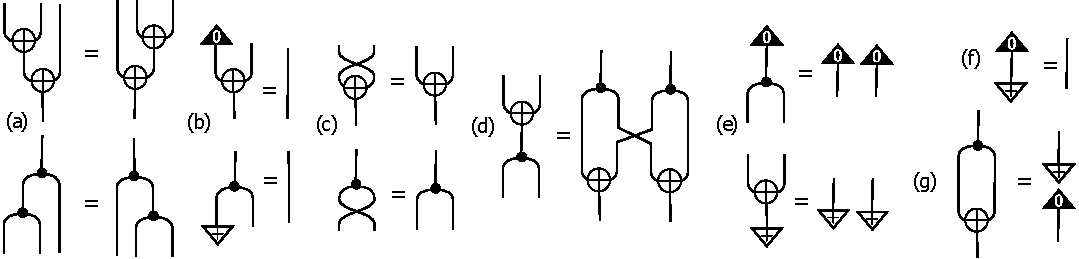
\includegraphics{F2-presentation1}
\end{center}
\end{illexample}
\end{myfullpage}



\begin{remark}[Alternative approaches to the linear fragment]\label{remark:related-work}
The structures in Figure \ref{fig:F2-presentation} which are found by casting classical circuits into tensor networks 
are used to form the building blocks needed to represent \CNOT{}-gates and are related to other approaches \cite{Kissinger09, DP10, Euler09} 
which have been used as a graphical language for measurement based quantum computation and for graph states \cite{DP10,Euler09}.
Our method of arriving at this collection of tensors (Figure \ref{fig:F2-presentation}) affords more general options and our presentation of the linear fragment 
here offers (i) improved semantics and (ii) a better theoretical understanding by pinpointing precisely that these networks correspond to the so called linear fragment 
of the \XOR{} or mod sum algebra carries with it new proof techniques.  These results were found by casting the theory of classical networks into a theory of tensors, 
which carried with it all of the known and desirable graphical rewrite properties from classical networks, and from this and some other methods, in \cite{CTNS} we 
assert that we have subsumed the existing graphical languages present in quantum information science by considering the 
the graphical system appearing in Figure \ref{fig:extraF2} together with the linear fragment from Figure \ref{fig:F2-presentation}.   
\end{remark}

\begin{myfullpage}
\begin{illexample}
\label{fig:extraF2}

%\begin{figure}[ht]
\begin{center}
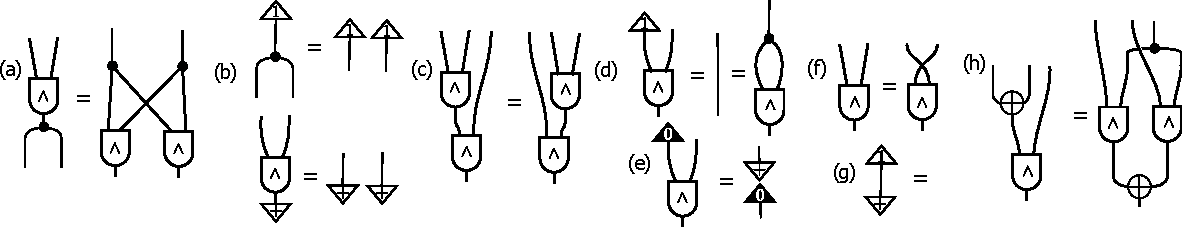
\includegraphics[width=\textwidth]{extra-F2-presentation1}
\end{center}
%\caption{
A summary of the quantum \AND-tensor calculus we apply to quantum information processing and tensor networks (reproduced from Lafont \cite{boolean03} and written to match the common quantum circuit notation as in \cite{CTNS}).  This figure with 
Figure~\ref{fig:F2-presentation} is a summary of the Boolean-calculus. 
The details of (a)-(g) will be given in
Sections~\ref{sec:components}.  For
instance, (h) represents distributivity of \AND{}($\wedge$) over \XOR{} ($\oplus$),
and (d) shows that $x\wedge x = x$. (Diagrams read top to bottom.)
%\end{figure}
\end{illexample}
\end{myfullpage}




\paragraph{Bending wires.}  Proceeding axiomatically we need to add additional tensors
to represent operators and quantum states. Our network model of quantum states
requires that we are able to bend wires.  As is well known in modern algebra, we 
can hence define transposition graphically (see Figure~\ref{fig:adjoints} (d)). Cups and caps (wire bending) was also used in the categorical model of teleportation \cite{catQM}---see also the early work on graphical representations of atemporal circuits \cite{Atemp06} and the diagramatic model of teleportation therein.  

The way forward is to add what mathematicians refer to as \textit{compact
structures} (see \S~\ref{sec:bends} for further 
details).  These compact structures are given diagrammatically as
\begin{center}
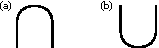
\includegraphics[width=5\xxxscale]{cup_and_cap}
%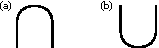
\epsfig{figure=cup_and_cap,width=5cm}
\end{center}
and as will be explored in \S~\ref{sec:bends} these two structures allow us to
formally bend wires and to define the transpose of a linear
map/state, and provide a formal way to reshape a matrix.  We understand (a) above as
a cup, given as the generalized
Bell-state 
\be 
\sum_{i=0}^{d-1}\ket{ii}= \ket{00}+\ket{11}+...
\ee 
and (b) above as the so-called cap, Bell-costate
\be 
\sum_{i=0}^{d-1}\bra{ii}=\bra{00}+\bra{11}+...
\ee 
or \textit{effect}.

\begin{remark}[Normalization factors omitted]
As we have mentioned before, we will often omit global scale factors (contracted tensor
networks with no open wires are sent to blank on the page).  This is done for ease of presentation.  We note that for Hilbert space $\2 H$ there is a natural isomorphism
\begin{equation*}
\7 C\otimes \2 H \cong \2 H \cong \2 H\otimes \7 C,
\end{equation*}
which allows one to define equality up to a scale factor (called the scalar gauge).  Care must be taken when summing over diagrams where a relative scale factor could exist. 
\end{remark}


As readers will recall from \S~\ref{sec:tensor}, compact structures provide a formal way to bend wires --- indeed, we can now connect a diagram represented with an operator with spectral decomposition 
$$
\sum_i
\beta_i\ket{i}\bra{i},
$$ 
bend all the open wires (or legs) towards the same direction
and it then can be thought of as representing a state 
$$
\sum_i \beta_i\ket{i}\ket{\overline{i}},
$$ 
where overbar is complex conjugation), bend them
the other way and it then can be thought of as
representing a measurement outcome 
$$
\sum_i
\beta_i\bra{\overline{i}}\bra{i}, 
$$
that is an effect.  One
can also connect inputs to outputs, contracting indices and creating larger and
larger networks. With these
ingredients in place, let us now consider the class of Boolean quantum states.

\begin{remark}[Overbar notation]
The isomorphism 
\begin{equation}
    \sum_i \beta_i\bra{\overline{i}}\bra{i}\cong \sum_i
\beta_i\ket{i}\bra{i} \cong \sum_i
\beta_i\ket{i}\ket{\overline{i}},
\end{equation}
for a real valued basis becomes
\begin{equation}
    \sum_i
\beta_i\bra{i}\bra{i}\cong \sum_i
\beta_i\ket{i}\bra{i} \cong \sum_i
\beta_i\ket{i}\ket{i},
\end{equation}
which amounts to flipping a bra to a ket and vise versa.  Here we will always assume a real valued 
basis so will always omit the overbar on kets.  
\end{remark}


\subsection*{Defining the class of Boolean tensor network states}\label{sec:c}
Figure \ref{fig:andtensor} which depicts a simple but
key network building block: the use of the so-called ``quantum \AND-tensor'' which we consider in detail in \S~\ref{sec:AND}.  This is a representation of
the familiar Boolean operation in the bit pattern of a three-qubit quantum state as
\begin{equation*}
\ket{\psi_\AND} \bydef
\sum_{x_1,x_2\in\{0,1\}}\ket{x_1}\otimes\ket{x_2}\otimes\ket{x_1\wedge
x_2}=\ket{000}+\ket{010} +\ket{100} +\ket{111},
\end{equation*}%\label{eqn:ANDstates}
and hence the truth table of a function is encoded in the bit pattern of the
superposition state. This utilizes a representation
of Boolean gates on quantum states.

\begin{figure}[t]
\centering
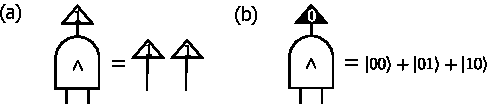
\includegraphics[width=12\xxxscale]{AND-intro}
%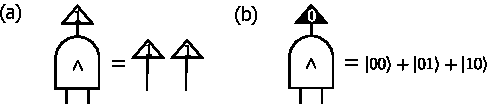
\epsfig{figure=AND-intro,width=12cm}
\caption{Example of the Boolean quantum \AND-state or tensor from \cite{CTNS}.  In (a) the
tensors output is contracted with $\bra{1}$ resulting in the tensor splitting to 
the product state $\ket{11}$.  In (b) the tensors output is contracted with $\bra{0}$ resulting in the entangled state
$\ket{00}+\ket{01}+\ket{10}$.}\label{fig:andtensor}
\end{figure}




We desire to construct tensor networks with components that take binary values $0$ or $1$.  This is done by contracting the output of a switching tensor network with $\ket{1}$.  The function realized in the tensor network is constructed in such a way that 
any time the input qubits states represent a
desired term in a quantum state
(e.g.\ create a function that outputs logical-one on designated inputs
$\ket{00}$, $\ket{01}$ and $\ket{10}$ and zero otherwise as shown in Figure
\ref{fig:andtensor}). We then insert a $\ket{1}$
at the network output.  This procedure
recovers the desired Boolean state as illustrated in Figure \ref{fig:bs}(a) with the
resulting state appearing in~\eqref{eqn:Booleaninput}.  
\be \label{eqn:Booleaninput}
\begin{aligned}
&\sum_{x_1,x_2,...,x_n\in\{0,1\}}\braket{1}{f(x_1
, x_2 ,...,x_n)}\ket{x_1,x_2,...,x_n} =\\ &\sum_{x_1,x_2,...,x_n\in\{0,1\}}f(x_1
, x_2 ,...,x_n)\ket{x_1,x_2,...,x_n}.
\end{aligned}
\ee 
The network representing the circuit is read backwards from output to
input.  Alternatively the full class of Boolean states is defined as:

\begin{definition}[The Class of Boolean Quantum States]
We define the class of Boolean states as those states which can be
expressed up to a global scalar factor in the form \eqref{eqn:Booleanstates}
\begin{equation}\label{eqn:Booleanstates}
\sum_{x_1,x_2,...,x_n\in\{0,1,...,d-1\}}\ket{x_1,x_2,...,x_n}\ket{f(x_1
, x_2 ,...,x_n)},
\end{equation} 
where 
$$
f:\{0,1\}^n\rightarrow \{0,1\},
$$
is a switching function and the sum is
taken over all variables $x_j$ taking 0 and 1 for qubits (see Figure \ref{fig:bs} (a)).  
\end{definition}

\begin{remark}[Better notation]
 In practice it is often simpler to express equations such as 
 \be 
 \sum_{x_1,x_2,...,x_n\in\{0,1\}}f(x_1, x_2,...,x_n)\ket{x_1,x_2,...,x_n},
\ee 
as 
\be 
\sum_{\textbf{x}} f(\textbf{x})\ket{\textbf{x}},
\ee 
where the sum is over all assignments of $\textbf{x}:= x_1,x_2,...,x_n$.  
\end{remark}

\begin{figure}[ht]
\centering
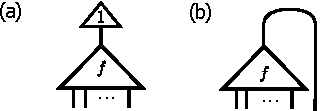
\includegraphics[width=7\xxxscale]{Boolean-state1}
%\epsfig{figure=Boolean-state,width=7cm}
\caption{A general Boolean quantum state arising from function $f$ can
either be formed as (a) by network contraction with a logical-one at the output of the circuit as
described by~\eqref{eqn:Booleaninput} or (b) by bending the output of the
tensor network around, as in~\eqref{eqn:Booleanstates}.}\label{fig:bs}
\end{figure}




\begin{fullpage}

\begin{example}[{\sf GHZ}-states and \W-states]
 Examples of Boolean states include the familiar {\sf GHZ}-state
$\ket{00\cdots0}+\ket{11\cdots1}$ which on qudits in dimension $d$ becomes 

\begin{equation}
 \ket{{\sf GHZ}_d}= \sum_{i=0}^{d-1} \ket{i}\ket{i}\ket{i} =
\ket{0}\ket{0}\ket{0}+\ket{1}\ket{1}\ket{1}+\cdots+\ket{d-1}\ket{d-1}\ket{d-1}, 
\end{equation}
as well as the \W-state
$\ket{00\cdots1}+\ket{01\cdots0}+\cdots+\ket{10\cdots0}$ which again on qudits
becomes
\be
\begin{aligned}\label{eqn:w-stated}
&\ket{\W_d} := \sum_{i=1}^{d-1} \sum_{j=1}^{3} (X_j)^i\ket{0}\ket{0}\ket{0} =
\ket{0}\ket{0}\ket{1}+\ket{0}\ket{1}\ket{0}+\ket{1}\ket{0}\ket{0}+\ket{0}\ket{0}\ket{
2}+\\
&\ket{0}\ket{2}\ket{0}+
\ket{2}\ket{0}\ket{0}+\cdots \cdots+\ket{0}\ket{0}\ket{d-1}+\ket{0} \ket{d-1}\ket{0} +\ket{d-1}\ket{0}\ket{0}. 
\end{aligned}
\ee

In~\eqref{eqn:w-stated} the operator
$X\ket{m}=\ket{m+1(\text{mod}~d)}$ is
one way to define negation in higher dimensions \cite{BB11}.  The subscript labels the ket
(labeled 1,2 or 3 from left to right) the operator acts $i$ times.
\end{example}
\end{fullpage}
\begin{remark}[Extensions to arbitrary quantum states]
What is clear from this definition is that Boolean states are always composed of equal
superpositions of sets of computational basis states, as the allowed scalars take binary values, 0,1. 
Despite this apparent limitation,
tensor networks composed only of Boolean components can nonetheless describe
any quantum state. To do this we require a minor extension to include superposition
input/output states, e.g. order-1 tensors of the form
$\ket{0}+\beta_1\ket{1}+\cdots+\beta_{d-1}\ket{d-1}$. This
gives a universal class of generalized Boolean tensor networks
which subsumes the important subclass of Boolean states.
This class is then shown to form a nascent example
of the exhaustiveness of BTNS and to give rise to a wide class of
quantum states that we show are exactly and efficiently sampled \cite{CTNS}.   
\end{remark}


 \begin{remark}[Comparison to other approaches]
  The theory of tensor network states has received recent interest fueled by developments that have been made related to 
  the important problem of quantum simulation, using tensor contraction algorithms \cite{MPSreview08,TNSreview09}. There is also an established language of quantum circuits, appearing in most text books on quantum computing and quantum information.  These circuits 
  are effectively tensor networks and efforts have been made to form an extension and unite the two \cite{BB11}.  
 \end{remark}


\section{Quantum Legos: a tensor tool box}\label{sec:components}
A key point to this is that the introduction of Boolean logic gate tensors
into the tensor network context allows the seminal logic gate universality results from classical network
theory to be applied in the setting of tensor network states. 

\begin{remark}[Dual spaces]
Any vector space $\2V$ has a dual $\2V^*$: this is the space of linear functions $f$
from $\2V$ to the ground field $\7C$, that is $f: \2V \rightarrow \7C$. This defines
the dual uniquely.  We must however fix a basis to identify the vector
space $\2V$ with its dual.  Given a basis, any basis vector $\ket{i}$ in $\2V$ gives
rise to a basis vector $\bra{j}$ in $\2V^*$ defined by $\braket{j}{i} = \delta^j_i$ (Kronecker's delta). 
This defines an isomorphism $\2V\rightarrow \2V^*$ sending $\ket{i}$ to $\bra{i}$ and
allowing us to identify $\2V$ with $\2V^*$.  In what follows, we will fix a particular
arbitrarily chosen basis (called the computational basis in quantum information
science).  We will now concentrate on Boolean building blocks that are used
in our construction.  
\end{remark}

% As we have mentioned in Remark \ref{remark:related-work}, the graphical language appearing in the 
% linear fragment (Figure \ref{fig:F2-presentation}) was considered first by Lafont \cite{boolean03} as well as in other work \cite{Kissinger09, DP10, Duncan2010, Euler09,redgreen, CTNS}.  The \AND-tensor and the connection to 
% Toffoli gates appeared first in \cite{CTNS}.  


\subsection*{Review of Boolean algebra}

Here we have reviewed Boolean tensor building blocks.  These building blocks appear in many applications of tensor network algorithms, including \cite{tommy}. Here we encourage the readers to review 
Boolean algebra to better understand the presented structures.  
We advise readers to quickly review Appendix \ref{sec:XOR} on \XOR-algebra as well as 
Appendix \ref{appendix:kmap} on the method of Karnaugh map equation reduction.  The following sections
will assume these methods are known to the reader.  


\subsection{{\sf COPY}-tensors: the ``diagonal''}\label{sec:COPY}

The copy operation arises in digital circuits~\cite{Davio78, Weg87}
and more generally, in the context of category theory and algebra, where it is
called a diagonal \cite{CD, redgreen}. The
operation is readily defined in any finite dimension as
\begin{equation}
\bigtriangleup \bydef \sum_{i=0}^{d-1} \ket{ii}\bra{i}.
\end{equation}
As $\ket{0}$ and
$\ket{1}$ are
eigenstates of $\sigma^z$, we might give $\bigtriangleup$ the alternative name of
{\sf Z}-copy.  In the
case of qubits {\sf COPY} is
succinctly presented by considering the map $\bigtriangleup$ that copies
$\sigma^z$-eigenstates:
$$
\bigtriangleup:\7C^2\rightarrow\7C^2\otimes\7C^2:
\begin{cases}
\ket{0} \mapsto \ket{00}\\
\ket{1} \mapsto \ket{11}
\end{cases}
$$
This map can be written in operator form as $\bigtriangleup:\ket{00}\bra{0} +
\ket{11} \bra{1}$ and
under cup/cap induced duality (on the right bra) this state becomes a {\sf GHZ}-state
as
$\ket{\psi_{\sf GHZ}} = \ket{000} + \ket{111}\cong\ket{00}\bra{0} +
\ket{11} \bra{1}$. The standard properties of {\sf COPY} are
given diagrammatically in Figure~\ref{fig:copygate} and a list of its relevant
mathematical properties are found in Table~\ref{fig:copygatesum}.

%\begin{myfullpage}
\begin{illexample}
\label{fig:copygate}
\begin{center}
%\begin{figure}[ht]
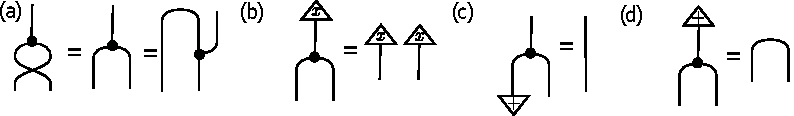
\includegraphics[width=.95\textwidth]{black-copy1}
\end{center}
%\caption{
Some diagrammatic properties of the {\sf COPY}-tensor. (a) Full-symmetry.
(b) Copy points, e.g.\ $\ket{x}\mapsto\ket{xx}$ for $x=0,1$ for qubits.  (c) The unit --- in this case
the unit corresponds to deletion, or a map to the
terminal object which is given as $\bra{+}\bydef\bra{0}+\bra{1}$ for qubits and
$\bra{+}\bydef\bra{0}+\bra{1}+\cdots+\bra{d-1}$ for $d$
dimensional qudits.  (d) Co-interaction with the unit creates a Bell state.
%\end{figure}
\end{illexample}
%\end{myfullpage}


\begin{remark}[The {\sf COPY}-gate from \CNOT]
The \CNOT-gate is defined as $\ket{0}\bra{0}_1\otimes \I_2 +
\ket{1}\bra{1}_1\otimes \sigma^x_2$.  We will set the input that the target acts on
to $\ket{0}$ then calculate $\CNOT (\I_1\otimes
\ket{0}_2)=\ket{0}\bra{0}_1\otimes \ket{0}_2 + \ket{1}\bra{1}_1\otimes
\ket{1}_2$.  We have hence defined the desired {\sf COPY} map copying states from the
Hilbert space with label $1$ (subscript) to the joint Hilbert space labeled $1$ and
$2$.   
\end{remark}

\begin{remark}[The types of possible states built from \COPY]
An alternative definition of the \COPY-tensor would be to define the operation by raising or lowering indices
 on $\delta^{ij}_{~~k}$, a Kronecker delta function.   
 In that regard, one might write the n-party \GHZ-state as 
 \be 
 \psi_\GHZ = \sum \delta^{ijk...l}\ket{ijk...l}.
 \ee 
Tensor products of state of this form are precisely the only types of states constructible with the \COPY-tensor alone.  
\end{remark}


\subsection{\XOR-tensors: the ``addition''}\label{sec:XOR}
The classical \XOR-gate implements exclusive disjunction or addition (mod 2 for
qubits) and is denoted by the
symbol $\oplus$~\cite{Cohn62, xor70}. We note that for multi-valued
logic a modulo subtraction gate can also be defined as in~\cite{BB11}.

\begin{remark}[relation to \COPY~\cite{CD, redgreen}]
 As is a well known fact in algebra, the \XOR-gate is simply a Hadamard
transform of the {\sf COPY}-gate, appropriately applied to all of the tensors
legs.  This can be captured diagrammatically in the slightly different form: 
\begin{center}
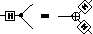
\includegraphics[width=0.250\textwidth]{dotduality}
\end{center}
\end{remark}

\begin{remark}[Symmetry]
 The \XOR-tensor is symmetric under leg exchange.  In components, if we write 
 $X_{ijk}$ then $X_{ijk}=1$ for $i=j=k=0$ (mod 2) and 0 otherwise.  
\end{remark}

To define the gate on the computational basis, we
consider $f(x_1,x_2)=x_1\oplus x_2$ then $f=0$ corresponds to
$(x_1,x_2)\in\{(0,0),(1,1)\}$ and $f=1$ corresponds to $(x_1,x_2)\in\{(1,0),(0,1)\}$,
where the
truth table for $\XOR$ follows. 
\begin{center}
% use packages: array
\begin{tabular}{c|c|c}
$~x_1~$ & $~x_2~$ & $f(x_1,x_2)=x_1\oplus x_2$ \\ \hline
0 & 0 & 0 \\
0 & 1 & 1 \\
1 & 0 & 1 \\
1 & 1 & 0
\end{tabular}
\end{center}
Under cap/cap induced duality, the state defined by $\XOR$ is given as
\begin{equation}
\ket{\psi_\oplus}\bydef\sum_{x_1,x_2\in\{0,1\}}\ket{x_1}\ket{x_2}\ket{f(x_1,x_2)}
=\ket { 000 }
+\ket { 110 }
+\ket{011}+\ket{101}, 
\end{equation}
which is in the {\sf GHZ}-class by LOCC equivalence viz.
$\ket{\psi_\oplus}=\H\otimes\H\otimes\H(\ket{000}+\ket{111})$.  The operation of
\XOR~is
summarized in Table~\ref{fig:xorgatesum}.  Since the
\XOR-gate is related to the {\sf COPY}-gate by a change of basis, its diagrammatic
laws
have the same structure as those illustrated in Figure~\ref{fig:copygate}.  The gate
acting backwards (co-\XOR) is
defined on a basis as follows:
$$
\oplus:\7C^2\rightarrow\7C^2\otimes\7C^2:
\begin{cases}
\ket{0} \mapsto \ket{00}+\ket{11}\\
\ket{1} \mapsto \ket{10}+\ket{01}
\end{cases}~~~~\text{or equivalently}~~~~~~~\begin{cases}
\ket{+} \mapsto \ket{++}\\
\ket{-} \mapsto \ket{--}
\end{cases}
$$



\subsection*{Generating the affine class of networks}
Thus far we have presented the {\sf XOR}- and {\sf COPY}- gates.  This system allows
us to create the linear class of Boolean functions.  As explained in the present
subsection, this class can be extended to to the affine class by introducing either a
gate that acts like an inverter, or by appending a constant $\ket{1}$ into our
system.  This constant will allow us to use the {\sf XOR}-gate to create an
inverter.   

\begin{definition}[Complemented vs uncomplemented Boolean variables]
A \textit{complemented Boolean variable} is a
Boolean variable that appears in negated form, that is $\neg x$ or
written equivalently as $\overline{x}$. Negation of a Boolean variable $x$ can be
expressed as the \XOR{} of
the variable with constant $1$ as $\overline{x}=1\oplus x$. Whereas
\textit{Uncomplemented Boolean
variables} are Boolean variables that do not appear in negated form (e.g.\ negation
is not allowed).  Linear Boolean functions contain terms with Uncomplemented Boolean
variables that
appear individually (e.g.\ variable
products are not allowed such as $x_1x_2$ and higher orders etc., see
\S~\ref{sec:Boolean}).   
\end{definition}


\begin{definition}[Linear Boolean functions]
Linear Boolean functions take the general form
\be
f(x_1,x_2,...,x_n)=c_1x_1\oplus c_2x_2\oplus ...\oplus c_nx_n,
\ee 
where the vector $(c_1,c_2,...,c_n)$ uniquely determines the function.   
\end{definition}

\begin{definition}[Affine boolean functions]
The affine
Boolean functions take the same general form as linear functions.  However, functions
in the affine class allows variables to appear in both complemented
and uncomplemented form. Affine Boolean functions take the general form
\begin{equation}\label{eqn:affine1}
f(x_1,x_2,...,x_n)=c_0\oplus c_1x_1\oplus c_2x_2\oplus ...\oplus c_nx_n,
\end{equation}
where $c_0=1$ gives functions outside the linear class.  From the identities,
$1\oplus 1=0$ and $0\oplus x=x$ we require the introduction of only one constant
($c_0$), see Appendix \ref{sec:Boolean}. 
\end{definition}

Together, \XOR{} and {\sf COPY} are not universal for classical circuits. When used
together, \XOR- and {\sf COPY}-gates compose to create networks representing the class of linear
circuits. The affine circuits are generated by considering the constant $\ket{1}$.
The state $\ket{1}$ is
indeed copied by the black tensor. However, our axiomatization
(Figure~\ref{fig:F2-presentation}) proceeds through 
considering the \XOR- and {\sf COPY}-gates together with $\ket{+}$, the unit for
{\sf COPY} and $\ket{0}$ the unit for \XOR.  It is by appending the constant
$\ket{1}$ into the
formal system (Figure~\ref{fig:F2-presentation}) that the affine class of circuits
can be realized.



\begin{remark}[Affine functions correspond to a basis]
Each affine function is labeled by a corresponding bit pattern.  This can be
thought of as labeling the computational basis, as
states of the form $\ket{\{0,1\}^n}$ are in correspondence with polynomials in
algebraic normal form (see Appendix \ref{sec:Boolean}).
\end{remark}

\subsection{Quantum \AND-state tensors: Boolean universality}\label{sec:AND}
The proceeding sections have introduced enough machinery to generate the linear and
affine classes of classical circuits.  These classes are not universal.  To recover
a universal system one will introduce the \AND{} gate as a tensor \cite{CTNS}.  The multiplicative unit for this gate is $\bra{1}$ and
so can be used to elevate the linear fragment to the affine class.  

The \AND{} gate (that is, $\wedge$) implements logical conjunction~\cite{Davio78,
Weg87}.  The \AND-gate relates to the \OR-gate via De
Morgan's law.
This can be captured diagrammatically as
\begin{center}
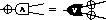
\includegraphics[width=0.35\textwidth]{demorgan}
\end{center}
To define the gate on the computational basis, we
consider $f(x_1,x_2)=x_1\wedge x_2$ which we write in short hand as $x_1 x_2$.  Here
$f=0$
corresponds to $(x_1,x_2)\in\{(0,0),(0,1),(1,0)\}$ and $f=1$ corresponds to
$(x_1,x_2)=(1,1)$. 


Under cap/cap induced duality, the state defined by $\AND$ is given as
\begin{equation}\label{eqn:quantumAND}
\ket{\psi_\wedge}\bydef\sum_{x_1,x_2\in\{0,1\}}\ket{x_1}\ket{x_2}\ket{f(x_1,x_2)}
=\ket { 000 }
+\ket { 010 }
+\ket{010}+\ket{111}.
\end{equation}
The key diagrammatic properties of {\sf AND}
are presented  in Figure~\ref{fig:ANDgate} and the gate is 
summarized in Table~\ref{fig:andgate}. 

The gate acting backwards (co-\AND) is
defined on a basis as follows: 

$$
\wedge:\7C^2\rightarrow\7C^2\otimes\7C^2:
\begin{cases}
\ket{0} \mapsto \ket{00}+\ket{01}+\ket{10}\\
\ket{1} \mapsto \ket{11}
\end{cases}~\text{or}~~\begin{cases}
\ket{+} \mapsto \ket{++}\\
\ket{-} \mapsto \ket{00}+\ket{01}+\ket{10} - \ket{11}
\end{cases}
$$

\begin{comment}
$$
\wedge:\7C^2\rightarrow\7C^2\otimes\7C^2:
\begin{cases}
\ket{0} \mapsto \ket{00}+\ket{01}+\ket{10}\\
\ket{1} \mapsto \ket{11}
\end{cases}~~~~~~~~~~~~~~~~~~~~~~~~~~
$$
$$~~~~~~~~~~~~~~~~~~~~~~~~~~~~~~~~~~~~~~~~~\text{or}~~~~~~~\begin{cases}
\ket{+} \mapsto \ket{++}\\
\ket{-} \mapsto \ket{00}+\ket{01}+\ket{10} - \ket{11}
\end{cases}
$$
\end{comment}


% Here: 
%\begin{myfullpage}
\begin{illexample}
 \label{fig:ANDgate}
Salient diagrammatic properties of the \AND-tensor.
\begin{center}
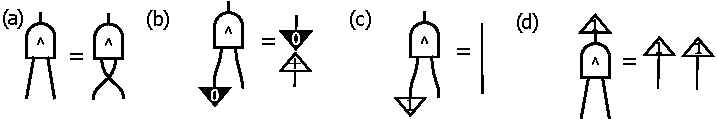
\includegraphics[width=0.95\textwidth]{AND1}
\end{center}
%\caption{
 (a) Input-symmetry. (b)
Existence of a zero or fixed-point.
(c) The unit $\ket{1}$.  (d) Co-interaction with the unit
creates a product-state.  Note that the gate forms a valid
quantum operation when run backwards as in (d).
%\end{figure}
 \end{illexample}
%\end{myfullpage}

\begin{example}[\AND-states from Toffoli-gates]\label{ex:ANDfromtoff}
The \AND-state is readily constructed from the Toffoli gate \cite{CTNS} as illustrated in
Figure~\ref{fig:ANDfromtoff}.  This allows some
interesting states to be created 
experimentally, for instance, post-selection of the output to $\ket{0}$
would yield the state $\ket{00}+\ket{01}+\ket{10}$. 
\end{example}

 \begin{remark}[Quantum universality and universal
states]\label{re:quantumuniversal}
 The problem of determining universal quantum gate families has received significant
 research interest resulting in the simplistic universal gate sets appearing
 in~\cite{A03,Shi:02,RG02} and elsewhere.  It is even known that Toffoli and Hadamard are
universal
 for quantum computation~\cite{A03}. Toffoli can be generated by combining one
 \AND-state and two {\sf COPY}-states (see also Figure \ref{fig:hadamard}).  \mn{In \cite{CTNS} the ZX calculus (Clifford gates plus cups and caps to bend wires) by considering the addition of \AND{}-states which can represent Toffoli gates was shown to be quantum computationally universal \cite{CTNS}.  With the addition of scalars, the \AND+ZX calculus presented in \cite{CTNS} was proven to be approximately universal  for linear maps between qubits.} 
 \end{remark}
 
 









\begin{theorem}[Toffoli contracts to give the \AND{}-state \cite{CTNS}]\label{fig:ANDfromtoff}
The following rewrites exhibit the use units to prepare the \AND-state \cite{CTNS}.  Using this state together with single qubit \NOT-gates, one can construct tensor networks which any Boolean qubit state as well as any of the states appearing in Table~\ref{fig:BooleanStates}.  We note that the box around the Toffoli gate (left) is meant to illustrate a
difference between our notation and that of quantum circuits.  In our notation, those dots inside the box would merge which of course is not a valid unitary gate.
\begin{center}
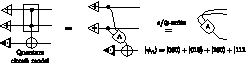
\includegraphics[width=0.95\textwidth]{tofftoand}
\end{center}
\end{theorem}



\begin{theorem}
 Hadamard follows from contracting the \AND-state 
together with $\ket{-}\bydef\frac{1}{\sqrt{2}}(\ket{0}-\ket{1})$ \cite{CTNS}.  
\begin{proof}
\begin{center}\label{fig:hadamard}
    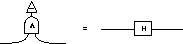
\includegraphics[width=9\xxxscale]{hadamard}
\end{center}
Follows by direct calculation. 
\end{proof}
\end{theorem}

\begin{definition}
 Hadamard
states are defined as 
$$
\ket{\psi_\H} = \ket{00}+\ket{01}+\ket{10}-\ket{11}. 
$$
\end{definition}

\begin{lemma}
Tensor contractions formed from Hadamard states, {\sf COPY}-and \AND-states are universal for quantum computation \cite{CTNS}. 
\begin{proof}
The proof \cite{CTNS} follows from wire bending duality and the proof that Hadamard and Toffoli are universal
for quantum circuits~\cite{A03}.
\end{proof}
\end{lemma}




\subsubsection{Summary of the {\sf XOR}-algebra on tensors}

We will now present the three previously referenced Tables (\ref{fig:copygatesum},
\ref{fig:xorgatesum} and \ref{fig:andgate}) which summarize the quantum logic tensors
we introduced in the previous subsections (\ref{sec:COPY}, \ref{sec:XOR} and
\ref{sec:AND}).  The tables contain entries listing properties that describe how
the introduced network components interact \cite{boolean03, CD, redgreen, CTNS, BB11}.  These interactions
are defined diagrammatically and explained in \S~\ref{sec:components}.  

\begin{center}
\begin{table}[ht]
\begin{tabular}{|c|c|c|c|}\hline
Gate Type & Co-copy point(s) & Unit & Co-unit Interaction\\\hline
{\sf COPY} & $\ket{0}$,$\ket{1}$  & $\ket{+}$  & Bell state: $\ket{00}+\ket{11}$
 \\ \hline\hline
Symmetry & Associative & Commutative & Frobenius Algebra\\\hline
Full  & Yes         & Yes & Yes (Fusion Law) \\ \hline
\end{tabular}
\caption{Summary of the {\sf COPY}-gate from \S~\ref{sec:COPY}.}\label{fig:copygatesum}
\end{table}
\end{center}

\begin{center}
\begin{table}[ht]
\begin{tabular}{|c|c|c|c|}\hline
Gate Type & Co-copy point(s) & Unit & Co-unit Interaction\\\hline
\XOR & $\ket{+}$,$\ket{-}$  & $\ket{0}$  & Bell state: $\ket{00}+\ket{11}$
 \\ \hline\hline
Symmetry & Associative & Commutative & Frobenius Algebra\\\hline
Full  & Yes         & Yes & Yes (Fusion Law) \\ \hline
\end{tabular}
\caption{Summary of the \XOR-gate from \S~\ref{sec:XOR}.}\label{fig:xorgatesum}
\end{table}
\end{center}

\begin{center}
\begin{table}[ht]
\begin{tabular}{|c|c|c|c|}\hline
Gate Type & Co-copy point(s) & Unit & Co-unit Interaction\\\hline
\AND & $\ket{1}$  & $\ket{1}$  & Product state: $\ket{11}$
 \\ \hline\hline
Symmetry   & Associative & Commutative & Bialgebra Law\\\hline
Inputs  & Yes         & Yes         & Yes (with {\sf GHZ}) \\ \hline
\end{tabular}
\caption{Summary of the \AND-gate from \S~\ref{sec:AND}.}\label{fig:andgate}
\end{table}
\end{center}


\subsection*{co-{\sf COPY}: the co-diagonal}\label{sec:co-diagonal}
What is evident from our subsequent discussions on logic gates is that in the context
of tensors, the bending of wires implies that gates can be used both forwards in backwards. We can therefore form tensor networks from Boolean gates
in a very
different way from classical circuits. Indeed, it becomes possible to flip a {\sf
COPY} operation upside down,
that is, instead of having a single leg split into two legs, have two legs merge into
one.  In
terms of tensor networks, co-{\sf COPY} is simply
thought of as being a dual (transpose) to the familiar {\sf COPY} operation. This is
common in
algebra: to consider the dual
notation to algebra, that is co-algebra.  In general, while a product is a joining or pairing (e.g.\ taking two
vectors and producing a third) a co-product is a co-pairing taking a single vector
in the space $\2A$ and producing a vector in the space $\2A\otimes \2 A$.

\begin{remark} [co-algebras~\cite{FA}]
co-algebras are structures that are dual (in the sense of
reversing arrows) to unital associative algebras such as {\sf COPY} and
\AND{} the axioms of which we formulated in terms of picture calculi
(Sections \ref{sec:COPY} and \ref{sec:AND}).  Every co-algebra, by
(vector space) duality, gives rise to an algebra, and in finite dimensions, this duality goes in both directions.  
\end{remark}

Co-{\sf COPY} can be thought of as applying a delta function in the transition from
input to output.  That is, given a copy point $x=0,1,...,d-1$ for qudits on dim $d$.
 Depicting {\sf COPY} as the map
$\bigtriangleup$
\begin{equation}
\bigtriangleup(\ket{x})=\ket{x}\otimes\ket{x},
\end{equation}
we define co-{\sf COPY} by the map $\bigtriangledown$ such that 
\begin{equation}
\bigtriangledown(\ket{i},\ket{j})=\delta_{ij} \ket{i},
\end{equation}
that is, the diagram is mapped to zero (or empty) if the inputs $\ket{i}$, $\ket{j}$
do not agree.  This is succinctly expressed in terms of a delta-function dependent on
inputs $\ket{i}$, $\ket{j}$ where $i,j=0,1,...,d-1$ for qudits of dim $d$.

\begin{example}[Simple co-pairing]
Measurement effects on tripartite quantum systems can be thought of as
co-products.  This is given as a map from one system (measuring the first) into two
systems (the effect this has on the other two). {\sf GHZ}-states are prototypical
examples of co-pairings.  In this case, the measurement outcome of $\ket{0}$
($\ket{1}$) on a single subsystem sends the other qubits to $\ket{00}$ ($\ket{11}$)
and by linearity this sends $\ket{+}$ to $\ket{00}+\ket{11}$.  
\end{example}

\subsection*{The remaining Boolean tensors: \NAND-states etc.}
We have represented a logical system on tensors --- this enables us
to represent any Boolean function as a connected network of tensors and hence any Boolean state.
We chose as our generators,
constant $\ket{1}$, {\sf COPY}, \XOR, \AND{}.  Other generators could have also been
chosen such as \NAND-tensors. Our choice however, was made as a matter of convenience. If we
had considered other generators, we could have ended up considering the
following cases: weak-units~(Definition \ref{def:weakunits}) and fixed point
pairs~(Definition \ref{def:fixedpoints}). 

% We note that the \NAND-states were used in \cite{1996quant.ph..5011S} for fault-tolerant quantum
% computation --- see also \cite{toffoli-state}.

\begin{definition}[Weak units]\label{def:weakunits}
An algebra (or product see Appendix \ref{sec:newalgebra}) on a tripartite state
$\ket{\psi}$ has a unit (equivalently, one has that the state is unital) if there
exists an effect $\bra{\phi}$ which
the product acts on to produce an invertible map $B$, where $B=\I$ (see
Example~\ref{ex:weakunits}). If no such $\bra{\phi}$ exists to make $B=\I$, and $B$
has an inverse, we call $\bra{\phi}$ a weak unit, and say the state $\ket{\psi}$ is
weak unital and if $B\neq \I$ and $B^2=1$ we call
the algebra on $\ket{\psi}$ unital-involutive.  This scenario is given
diagrammatically
as:
\begin{center}
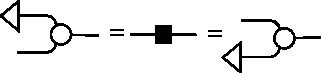
\includegraphics[width=6.5\xxxscale]{weak-unital}
%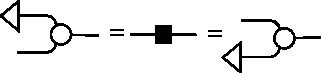
\epsfig{figure=weak-unital,width=6.5cm}
\end{center}
\end{definition}
\begin{example}[\NAND{} and \NOR{}]\label{ex:weakunits}
\NAND{} and \NOR{} have weak units, respectively given by $\ket{1}$ and $\ket{0}$.
These weak units are unital-involutive.
\begin{equation}
 \ket{\psi_\NAND} = \ket{001}+\ket{011}+\ket{101}+\ket{110},
\end{equation}
\begin{equation}
 \ket{\psi_\NOR} = \ket{001}+\ket{010}+\ket{100}+\ket{110}.
\end{equation}
For $\ket{\psi_\NAND}$ to have a unit, there must exist a $\ket{\phi}$ such that
\begin{equation}
 \braket{\overline{\phi}}{0}\ket{01}+\braket{\overline{\phi}}{0}\ket{11}+\braket{
\overline{\phi}}{1}\ket{01} +\braket{\overline{\phi}}{1}\ket{10}=\ket{00}+\ket{11},
\end{equation}
and hence no choice of $\ket{\phi}$ makes this possible, thereby confirming the
claim.
\end{example}

\begin{definition}[Fixed Point Pair]\label{def:fixedpoints}
An algebra (see Appendix \ref{sec:newalgebra}) on a tripartite state
$\ket{\psi}$ has a \textit{fixed point} if
there exists an effect $\bra{\phi}$ (the fixed point) which
the product acts on to produce a constant output, independent of the other input value. 
For instance, in Figure \ref{fig:fixedpoints}(c) on the left hand side the effect
$\bra{1}$ induces a map (read bottom to top) that sends $\ket{+}\mapsto \ket{1}$. 
Up to a scalar, this map expands linearly sending both basis effects $\bra{0}$,
$\bra{1}$ to to the constant state $\ket{1}$. If the resulting output is the same as
the fixed point, we say $\bra{\phi}$ has a zero ($\ket{1}$ is the zero for the
\OR-gate in Figure \ref{fig:fixedpoints}(c)). A
fixed point pair consists of two algebras with fixed points, such that the fixed
point of one algebra is the unit of the other, and vise versa (see
Figure~\ref{fig:fixedpoints}). Diagrammatically this
is given in Figure \ref{fig:fixedpoints2}.  
\end{definition}

\begin{figure}[ht]
\centering
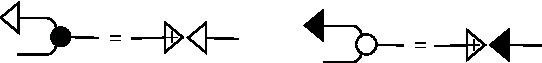
\includegraphics[width=11\xxxscale]{fixed-points}
%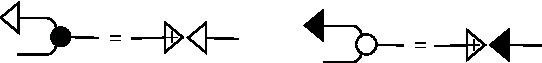
\epsfig{figure=fixed-points,width=11cm}
\caption{Diagrammatic equations satisfied by a fixed point
pair (see Definition \ref{def:fixedpoints}). }\label{fig:fixedpoints2}
\end{figure}

\begin{figure}[ht]
\centering
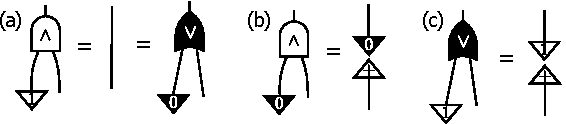
\includegraphics[width=11\xxxscale]{fixedpoints1}
%\epsfig{figure=fixedpoints,width=11cm}
\caption{\AND{} and \OR{} tensors form a fixed point pair.  The unit for \AND{}
($\ket{1}$
see a) is the zero for \OR{} (c) and vise versa: the unit of \OR{} ($\ket{0}$
see a) is the zero for \AND{} (b).}\label{fig:fixedpoints}
\end{figure}

\subsection*{Summarizing: network composition of quantum logic tensors}
We have considered sets of universal classical structures in our tensor
network model.  In classical computer science, a universal set of gates is able to
express any $n$-bit Boolean function
\begin{equation}
  f:\7B^n\rightarrow\7B:(x_1,...,x_n)\mapsto f(x_1,...,x_n),
\end{equation}
where we note that $\7Z_2\cong\7B$ allowing us to use the alternative notation for
$f$ as $f:\7Z_d^n\rightarrow\7Z_d$ with $d=2$ for the binary case. Universal sets
include
\begin{itemize}
    \item[1.] \{{\sf COPY}, \NAND\},
    \item[2.] \{{\sf COPY}, \AND,~\NOT\},
    \item[3.] \{{\sf COPY}, \AND,~\XOR, $\ket{1}$\},
    \item[4.] \{\OR,~\XNOR, $\ket{1}$\} and others.  
\end{itemize}
One can also consider the states $\ket{\psi}$ formed by the bit patterns of these functions $f(x_1,x_2)$ as
\be
\ket{\psi_f} = \sum_{x_1,x_2\in\{0,1\}}\ket{x_1}\ket{x_2}\ket{f(x_1,x_2)}.
\ee
This allows a wide class of states to be constructed effectively.  In the
following
Table (\ref{fig:BooleanStates}) we illustrate the quantum states representing the classical
function of two-inputs.


The bit pattern of the following quantum states represents a Boolean function (given by the subscript) such that the right most bit is the Boolean functions output, and the two left bits are the functions inputs, and the non-linear Boolean functions are
on the left side of the table and the linear functions on the right.  Consider the state $\ket{\psi_\AND}$, and Boolean variables $x_1$ and $x_2$, then the superposition $\ket{\psi_\AND}$ encodes the function $\ket{x_1,x_2,x_1\wedge x_2}$ in each term in the superposition, and
$$ 
\ket{\psi_\AND}=\sum_{x_1,x_2\in\{0,1\}}\ket{x_1,x_2,x_1\wedge
x_2}.
$$ 

As outlined in the text, cup/cap induced-duality allows us (for instance) to express this state as the operator
$$ 
\ket{0}\bra{00}+\ket{0}\bra{01}+\ket{0}\bra{01}+\ket{1}\bra{11}:\ket{x_1,x_2} \mapsto\ket{x_1\wedge x_2}
$$
which projects qubit states to the $\AND$ of their bit value.

\begin{center}
\begin{table}[ht]
% use packages: array
\begin{tabular}{|c|c|}\hline
non-linear & linear (Frobenius Algebras) \\\hline
$\ket{\psi_\AND}=\ket{000}+\ket{010}+\ket{100}+\ket{111}$ &  \\
~$\ket{\psi_\OR}=\ket{001}+\ket{011}+\ket{101}+\ket{111}$ &
~$\ket{\psi_\XOR}=\ket{000}+\ket{011}+\ket{101}+\ket{110}$\\
$\ket{\psi_\NAND}=\ket{001}+\ket{011}+\ket{101}+\ket{110}$ &
$\ket{\psi_\XNOR}=\ket{001}+\ket{010}+\ket{100}+\ket{111}$\\
~$\ket{\psi_\NOR}=\ket{001}+\ket{010}+\ket{100}+\ket{110}$ & \\\hline
\end{tabular}
\end{table}\label{fig:BooleanStates}
\end{center}



\subsubsection{Merging {\sf COPY}-tensors by node equivalence}
{\sf COPY}-tensors are readily generalized to an arbitrary number of input and
output legs. As one would rightly suspect,
a {\sf COPY}-tensor with $n$~inputs and $m$~outputs corresponds to an
$n+m$-partite {\sf GHZ}-state.  Neighboring tensors of the same type can be merged into
a single tensor: this is called node equivalence in digital circuits. {\sf
COPY}-tensors represent Frobenius algebras\mn{In the work \cite{COECKE_2012}, the \COPY{}-tensor, through its properties as a Frobenius algebra \cite{DP13}, was shown to be equivalently characterised by an orthogonal basis for a finite-dimensional Hilbert space.}~\cite{Carboni-Walters,FA}.

\begin{theorem}[Node equivalence or fusion law]\label{theorem:spider} Given a
connected graph with $m$~inputs and $n$~outputs comprised solely of \COPY-tensors of
equal dimension, this map
can be equivalently expressed as a single $m$-to-$n$ tensor, as shown as 
\begin{center}
    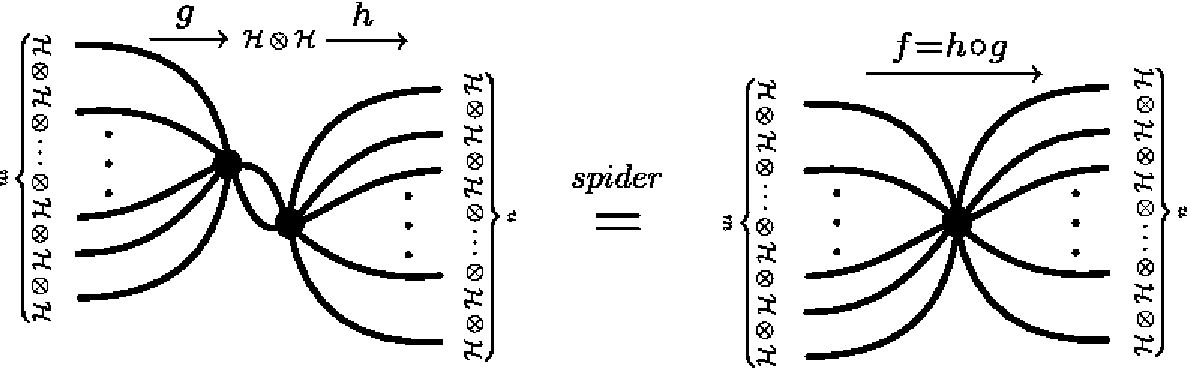
\includegraphics[width=0.95\textwidth]{joinspider}
\end{center}
Node equivalence or fusion law.  Connected black-tensors ($\bullet$) as well as connected plus-tensors
($\oplus$) can be merged and also split apart at will.  The intuition for digital or qudit circuits follows by connecting a state $\ket{\phi}$ to one of the legs and iterating over a complete basis $\ket{0}$, $\ket{1}$,...,$\ket{d-1}$.\\ 

This rule goes by many different names, depending on the community.  For example, in classical circuits this is called node equivalence whereas researchers in categorical quantum mechanics, credit node equivalence as their own {\it spider law} \cite{redgreen}. 
\label{fig:Spider}
\end{theorem}

\subsection*{Associativity, distributivity and commutativity}

The products we have considered are all associative and commutative.  As algebras,
\AND{}, \XOR{} and {\sf COPY}{} are associative, unital commutative algebras.  This
was
already expressed diagrammatically in Figures~\ref{fig:F2-presentation}(a) and
Figure \ref{fig:extraF2}(c).
The diagrammatic laws relevant for this subsection represent the following
Equations
\begin{equation}
(x_1\wedge x_2)\wedge x_3= x_1\wedge (x_2\wedge x_3),
\end{equation}
\begin{equation}
(x_1\oplus x_2)\oplus x_3= x_1\oplus (x_2\oplus x_3).
\end{equation}
Distributivity of \AND{} over \XOR{} then becomes (see (h) in
Figure~\ref{fig:extraF2})
\begin{equation}
(x_1\oplus x_2)\wedge x_3= (x_1\wedge x_2)\oplus (x_1\wedge x_2).
\end{equation}
We have commutativity for any product symmetric in its inputs: this is
the case for \AND{} and \XOR.

\subsection*{Bialgebras on tensors}\label{sec:bialgebra}
There is a powerful type of algebra that arises in our
setting: a bialgebra defined graphically on tensors in Figure
\ref{fig:BialgebraAxioms} (see Kassel, Chapter III~\cite{Kassel}, \cite{FA} and \cite{redgreen}).  

 Such an algebra is simultaneously a unital associative algebra and co-algebra (for
the associativity condition see (b) in Figure~\ref{fig:BialgebraAxioms}).
Specifically, we consider the following two ingredients:
\begin{description}\addtolength{\itemsep}{-0.5\baselineskip}
\item[(i)] A product (black tensor) with a unit (black triangle) see the right hand
side of Figure~\ref{fig:BialgebraAxioms}(a).
\item[(ii)] A co-product (white tensor) with a co-unit
(white triangle) see the left hand side of Figure~\ref{fig:BialgebraAxioms}(a). 
\end{description}
To form a bialgebra, these two ingredients above must be characterized by
the following four compatibility conditions:
\begin{description}\addtolength{\itemsep}{-0.5\baselineskip}
\item[(i)] The unit of the black tensor is a copy-point of the white tensor as in (e)
from Figure~\ref{fig:BialgebraAxioms}.
\item[(ii)] The (co)unit of the white tensor is a copy-point of the black tensor as in (d)
from Figure~\ref{fig:BialgebraAxioms}.
\item[(iii)] The bialgebra-law is satisfied given in (c) from
Figure~\ref{fig:BialgebraAxioms}.
\item[(iv)] The inner product of the unit (black triangle) and the co-unit (white
triangle) is non-zero (not shown in Figure~\ref{fig:BialgebraAxioms}).
\end{description}

\begin{figure}[ht]
\centering
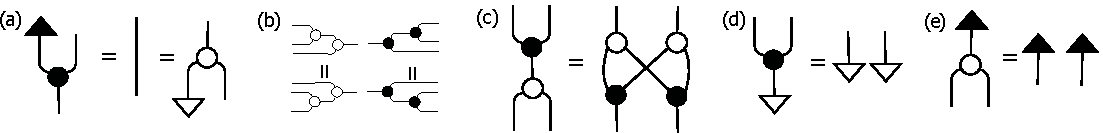
\includegraphics[width=0.95\textwidth]{bialgebraII1}
\caption{Bialgebra axioms~\cite{FA} (scalars are omitted).  (a) unit laws (these are
of course
left and right units); (b) associativity; (c) bialgebra; (d,e) co-{\sf COPY}
points.}\label{fig:BialgebraAxioms}
\end{figure}

\begin{example}[{\sf GHZ}, \AND{} form a bialgebra \cite{CTNS}]
We are in a position to study the interaction of {\sf GHZ}-\AND.   This interaction
satisfies the equations in Figure \ref{fig:BialgebraAxioms}: (a) the bialgebra law;
(b) the co-copy point of \AND{} is $\ket{1}$; and (c) the co-interaction with the
unit for {\sf GHZ} creates a compact structure.  In addition, (a) and (b) show the
copy points for the black {\sf GHZ}-tensor; in (c) we have the unit and fixed point
laws.
\end{example}

Even if a given product and co-product do not satisfy all of the compatibility
conditions (given in (a), (b), (c), (d), (e) in Figure \ref{fig:BialgebraAxioms}),
and hence do not form bialgebras, they can still satisfy the bialgebra law which is
given in Figure \ref{fig:BialgebraAxioms}(c).  Examples of states
that satisfy the bialgebra law in Figure \ref{fig:BialgebraAxioms}(c), but are not
bialgebras are given in Definition~\ref{def:bialgebra}. Notice that bialgebra
provides a highly constraining characterization of the tensors involved and is
tantamount to defining a commutation relation between them.

\begin{definition}[Bialgebra Law~\cite{FA}]\label{def:bialgebra}
A pair of quantum states (black, white tensors) satisfy the bialgebra law if (c)
in Figure \ref{fig:BialgebraAxioms} holds.  The Boolean states, \AND, \OR, \XOR,
\XNOR, \NAND, \NOR{} all satisfy the bialgebra law with {\sf COPY}.  
\end{definition}

\subsubsection{Algebras on valence-3 tensors}\label{sec:hopf}
A particularly important class of bialgebras are known as Hopf-algebras~\cite{FA}.
This is characterized by the way in which algebras and co-algebras can interact.  This
is captured by the Hopf-law, where the linear map $A$ is known as the antipode.

\begin{definition}[Hopf-Law~\cite{FA}]
A pair of quantum states satisfy the Hopf-Law if an $A$ can be found such that the
following equations hold:
\begin{center}
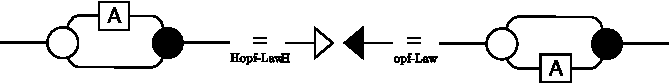
\includegraphics[width=12\xxxscale]{hopf-law}
%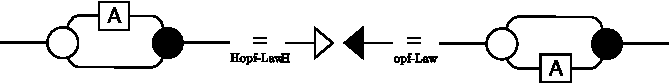
\epsfig{figure=hopf-law,width=12cm}
\end{center}
\end{definition}

\begin{example}[\XOR{} and {\sf COPY} are Hopf-algebras on Boolean States
\cite{boolean03}]
It is well known (see e.g.\ \cite{boolean03}) that the Boolean state \XOR, satisfies
the Hopf-algebra law with trivial antipode ($A=\I$) with {\sf COPY}.  Recall Figure
\ref{fig:F2-presentation}(g). 
\end{example}

\subsection*{Bending wires: compact structures}\label{sec:bends}
As mentioned in the preliminary section (\ref{sec:overview}), we make use of
what's called a \textit{compact structure} in category theory which amounts to
introducing cups and caps, to provide a formal way to bend wires and define
transposition. See Figures
\ref{fig:cupsetc} and \ref{fig:adjoints}.  

A \textit{compact structure} on an object $\2H$ consists of another object $\2H^*$
together with a pair of morphisms (note that we use the equation $\2H^*=\2H$ in
Hilbert space making objects self dual which simplifies what follows).
\begin{equation*}
  \eta_{\2H} : \7C \longrightarrow {\2H} \otimes {\2H}, ~~~~~~~~~~~~~~\epsilon_{\2H}
: {\2H} \otimes {\2H} \longrightarrow \7C,
\end{equation*}
where the standard representation in Hilbert space with dimension $d$ and basis
$\{\ket{i}\}$ is given by
\begin{equation*}
\eta_{\2H} = \sum_{i=0}^{d-1}\ket{i}\otimes\ket{i}, ~~~~~~~~~~~~~~ \epsilon_{\2H} =
\sum_{i=0}^{d-1}\bra{i}\otimes\bra{i},
\end{equation*}
and in string diagrams (read from the top to the bottom of the page) as
\begin{center}
  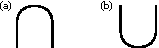
\includegraphics[width=0.25\textwidth]{cup_and_cap}
\end{center}
These cups and caps give rise to cup/cap-induced
duality: this amounts to being able to create a linear map that ``flips'' a bra to a
ket (and vise versa) and at the same time taking an (anti-linear) complex conjugate.
 In other words, the cap $\sum_{i=0}^1\bra{ii}$ sends  quantum state
$\ket{\psi}=\alpha\ket{0} + \beta\ket{1}$ to $\alpha\bra{0} + \beta\bra{1}$ which is
equal to the complex conjugate of $\ket{\psi}^\dagger =
\bra{\psi}=\overline{\alpha}\bra{0} + \overline{\beta}\bra{1}$.  Diagrammatically,
the dagger is given by mirroring operators across the page, whereas transposition is
given by bending wire(s). Clearly, $\bra{\overline{\psi}}=\alpha\bra{0} +
\beta\bra{1}$.  

In the case of relating the Bell-states and effects to the identity operator, under
cup/cap-induced duality, we flip the second ket on $\eta_{\2H}$ and the first bra on
$\epsilon_{\2H}$.  This relates these maps and the identity $\I_{\2H}$ of the
Hilbert space: that is, we can fix a basis and construct
invertible maps sending $\eta_{\2H}~\cong~\I_{\2H}~\cong~\epsilon_{\2H}$.  More
generally, the maps $\eta_{\2H}$ and $\epsilon_{\2H}$ satisfy the
equations given in Figure \ref{fig:cupsetc} and their duals
under the dagger. 

A second way to introduce cups and caps is to consider a \textit{Frobenius
form}~\cite{FA} on
either of the structures in the linear fragment from Figure \ref{fig:F2-presentation}
({\sf COPY} and \XOR).  This is simply a functional that turns a
product/co-product into a cup/cap.  This allows one to recover the above compact
structures (that is, the cups and caps given above) as
\begin{center}
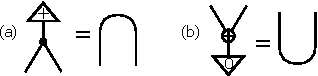
\includegraphics[width=7\xxxscale]{compactII}
%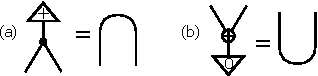
\epsfig{figure=compactII,width=6cm}
\end{center}
Again, we will use these cups and caps as a formal way to bend wires in tensor
networks: this can be thought of simply as a reshape of a matrix.

\begin{figure}[ht]
\centering
  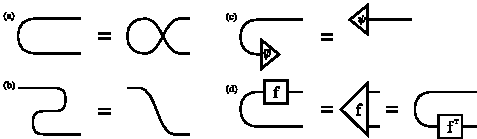
\includegraphics[width=0.7\textwidth]{cups}
\caption{Cup identities. (a) Symmetry. (b) Conjugate state.
(c) the \textit{snake equation}.
(d) Sliding an operator around a cup transposes it.}\label{fig:cupsetc}
\end{figure}


\begin{figure}[ht]
\centering
  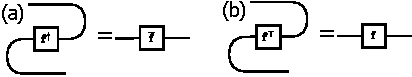
\includegraphics[width=0.7\textwidth]{dagger2}
\caption{Diagrammatic adjoints.  Cups and caps allow
us to take the transpose of a
linear map.  Note that care must be taken, as flipping
a ket $\ket{\psi}$ to a bra $\bra{\psi}$ is conjugate
transpose, and bending a wire is simply transposition, so the conjugate must be
taken: e.g.\ acting on $\ket{\psi}$ with a cap given as $\sum_i \bra{ii}$ results in
$\bra{\overline \psi}$.  }\label{fig:adjoints}
\end{figure}

\section{Examples of Boolean Tensor Network States}\label{sec:CTN}


\subsection*{Constructing Boolean states}\label{sec:W}
Since the fixed building blocks of our tensor networks are the logic tensors \AND,
\OR,
\XOR\, and {\sf COPY}, along
with ancilla bits, we can immediately apply the universality of these elements for classical circuit construction
to guarantee that any Boolean state has a tensor network decomposition.
However our construction goes beyond this because as we have seen,
Boolean tensor networks can be deformed and rewired in ways which are not
ordinarily permitted in the standard acyclic-temporal definition of classical
circuits. The \W-state will be shown to provide a non-trivial example of this.

\begin{example}[Functions on \W- and {\sf GHZ}-states]\label{ex:WandGHZ}
We consider the function $f_\W$ which outputs logical-one given input bit string
$001$, $010$ and $100$ and logical-zero otherwise.  Likewise the function
$f_{{\sf GHZ}}$ is defined to output logical-one on input bit strings $000$ and $111$
and
logical-zero otherwise.  See Examples \ref{ex:WandGHZBoolean} and
\ref{ex:mlWandGHZ} which
consider representation of these functions as polynomials.  We will continue to work
with a linear representation of functions on quantum states; here
bit string
$000\mapsto \ket{000}$ (etc.).
\end{example}

\begin{example}[MPS form for \W-state]
Like the {\sf GHZ} state, the \W-state has a
simple MPS representation
\be\label{eqn:wnMPS}
\ket{\W_n} = \bra{0}\left( \begin{array}{cc}
\ket{0} & 0 \\
\ket{1} & \ket{0} \end{array} \right)^{n}\ket{1}=
\ket{10...0}+\ket{01...0}+...+\ket{00...1}.
\ee
This description \eqref{eqn:wnMPS} is succinct.   All MPS-states have essentially this 
same topological or network structure. In contrast, our
categorical construction
described below breaks this network up further.
\end{example}

\begin{remark}[Exact-value functions]
The function $f_\W$ takes value logical-one on input vectors with $k$ ones for a
fixed integer $k$.
Such functions are known in the literature as Exact-value symmetric Boolean
functions.  When cast into our framework, exact-value functions give
rise to tensor networks which represent what are known as Dicke states
\cite{2010NJPh...12g3025A}. 
\end{remark}

\begin{example}[Function realization of $f_\W$ and
$f_{{\sf GHZ}}$: the Boolean case]\label{ex:WandGHZBoolean}
One can express (using $\overline x$ to mean Boolean variable negation)
\begin{equation}
f_\W(x_1,x_2,x_3)=\overline x_1\overline x_2x_3\oplus
x_1\overline x_2\overline x_3\oplus \overline x_1x_2\overline x_3
\end{equation}
by noting that each term in the disjunctive normal form of $f_\W$ are disjoint, and
hence \OR~maps to \XOR~as $\vee\mapsto \oplus$.  The algebraic normal form (see
Appendix~\ref{sec:Boolean}) becomes
\begin{equation}\label{eqn:fWBoolean}
f_\W(x_1,x_2,x_3)=x_1 \oplus x_2\oplus x_3\oplus x_1 x_2 x_3
\end{equation}
\begin{equation}
f_{{\sf GHZ}}(x_1,x_2,x_3) =1\oplus x_1\oplus x_2\oplus x_3\oplus x_1 x_2\oplus
x_1x_3\oplus x_2x_3
\end{equation}
\end{example}

\begin{example}[Function realization of $f_\W$ and $f_{{\sf GHZ}}$: the set
function case] \label{ex:mlWandGHZ}
Set functions are mappings from the family of subsets of a finite ground set (e.g.\
Booleans) to the real or complex numbers.  In the circuit theory literature,
functions from the Booleans to the reals are known as pseudo-Boolean functions and
more commonly as
multi-linear polynomials or forms (see~\cite{JDB08} where these functions are used to
embed a co-algebraic theory of logic gates in the ground state energy configuration of
spin models). There exists an algebraic normal form and hence a unique multi-linear
polynomial representation for each pseudo-Boolean
function (see Appendix~\ref{sec:Boolean}).  This is found by mapping the negated
Boolean variable as
$\overline{x}\mapsto
(1-x)$.  For the {\sf GHZ}- and \W-functions defined in Example~\ref{ex:WandGHZ} we
arrive
at the unique polynomials \eqref{eqn:mlGHZ} and \eqref{eqn:mlW}.
\begin{equation}\label{eqn:mlGHZ}
f_{{\sf GHZ}}(x_1,x_2,x_3)=1 - x_1 - x_2 + x_1 x_2 - x_3 + x_1 x_3 + x_2 x_3
\end{equation}
\begin{equation}\label{eqn:mlW}
f_{\W}(x_1,x_2,x_3) = x_1 + x_2 + x_3 - 2 x_1 x_2 - 2 x_1 x_3 - 2 x_2 x_3 + 3 x_1
x_2 x_3
\end{equation}
These polynomials \eqref{eqn:mlGHZ} and \eqref{eqn:mlW} are readily translated into
Boolean tensor networks.
\end{example}

\begin{example}[Network realisation of \W- and {\sf GHZ}-states]
A network realization of \W- and {\sf GHZ}-states in our framework then follows by
post-selecting the relevant network to $\ket{1}$ on the output bit --- leaving the
input qubits to
represent a \W- or {\sf GHZ}-state respectively. An example of this is shown in
Figure~\ref{fig:Wfunction}.
\end{example}


\begin{figure}[ht]
\centering
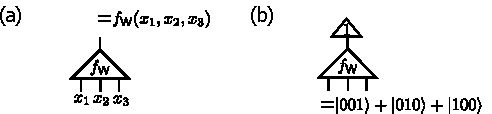
\includegraphics[width=14\xxxscale]{W-function1}
%\epsfig{figure=W-function,width=14cm}
\caption{Left (a) the circuit realization (internal to the triangle) of the function
$f_\W$ of e.g.\ \eqref{eqn:fWBoolean} which outputs logical-one given input $\ket{x_1
x_2 x_3}=$ $\ket{001}$, $\ket{010}$ and $\ket{100}$ and logical-zero
otherwise. Right (b) reversing time and setting the output to $\ket{1}$ (e.g.\
post-selection) gives a network representing the \W-state.  The na\"{i}ve
realization of $f_\W$ is given in Figure~\ref{fig:CategoricalWStates}
with an optimized co-algebraic construction shown in Figure
\ref{fig:CategoricalWStates}.}\label{fig:Wfunction}
\end{figure}

\begin{figure}[ht]
\centering
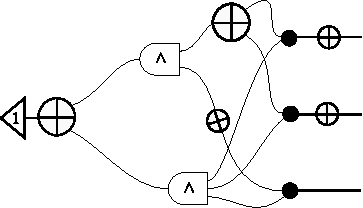
\includegraphics[width=7\xxxscale]{W-circuit-classical}
%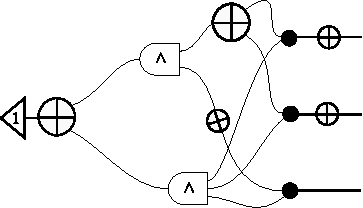
\epsfig{figure=W-circuit-classical,width=7cm}
\caption{Na\"{i}ve BTNS realization of the familiar \W-state
$\ket{001}+\ket{010}+\ket{100}$.  A standard (temporal) acyclic classical circuit
decomposition in terms of the \XOR-algebra realizes the function $f_\W$ of three
bits.  This function is given a representation on tensors.  As illustrated, the
networks input
is post selected to $\ket{1}$ to realize the desired
\W-state.}\label{fig:temporalWStates}
\end{figure}

\begin{figure}[ht]
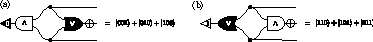
\includegraphics[width=15\xxxscale]{W-and-or}
%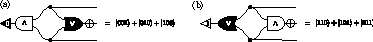
\epsfig{figure=W-and-or,width=15cm}
\caption{\W-class states in the Boolean tensor network state formalism.  (a)
is the standard \W-state.  (b) is found from applying De Morgan's law (see
\S~\ref{sec:AND}) to (a) and rearranging after inserting inverters on the output
legs. Notice the atemporal nature of the circuits, as
one gate is used forwards, and the other backwards.}\label{fig:CategoricalWStates}
\end{figure}

Two different Boolean tensor constructions for the building blocks of the \W-state are shown
in Figure~\ref{fig:temporalWStates} and  Figure~\ref{fig:CategoricalWStates}. Notice that in Figure~\ref{fig:CategoricalWStates} the
resulting tensor network forms an atemporal classical circuit and is much more efficient than
the na\"{i}ve construction in Figure~\ref{fig:temporalWStates}. Moreover by
appropriately daisy-chaining the networks in
Figure~\ref{fig:CategoricalWStates} we construct a Boolean tensor network for
an $n$-party \W-state
as shown in Figure~\ref{fig:nPartyCategoricalWStates}. Contrast this with other factorizations appearing in the literature~\cite{Kissinger09}. The resulting form of this tensor network is entirely equivalent
(up to regauging) to the MPS description given earlier, but now reveals internal structure of the state in terms of BTNS building blocks.

\begin{figure}[ht]
\begin{center}
  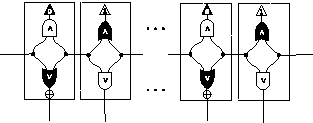
\includegraphics[width=14\xxxscale]{n-bits-W-and-or}  
\end{center}
%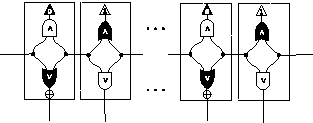
\epsfig{figure=n-bits-W-and-or,width=14cm}
\caption{\W-state ($n$-party) in the Boolean tensor network state formalism. The comb-shaped feature of efficient network contraction remains, with the internal structure of the network components exposed in terms of well understood algebraic structures.}\label{fig:nPartyCategoricalWStates}
\end{figure}


\section{Discussion} 

We have introduced a class of quantum states, known as Boolean quantum states.  This class is of interest, since it allows one to study quantum states using the well understood Boolean algebra.  In addition, states in this class have an evident tensor network.  

\begin{theorem}[The Class of Boolean Quantum States \cite{CTNS}]
 Every switching function $f(\x)$ gives rise to a quantum state with binary coefficients in $\{0,1\}$.  Moreover, a tensor network 
 representing this state is determined from the classical network description of $f(\x)$.  
\end{theorem}

\begin{remark}[From composition to contraction]
The quantum tensor network is found by letting each classical gate act on a linear space and from changing the composition of functions, to the contraction of tensors.
\end{remark}

\begin{remark}[Shannon and Davio decomposition]
 There are several elegant methods that allow one to factor a classical function into networks of different structures.  We should only have time to briefly mention these.  Those interested can consult wikipedia for Shannon and Davio decompositions.  
\end{remark}

We have examined in some detail a Boolean tensor tool box.  This is perhaps the most accessible part of tensor network states, due to its strong relation to Boolean circuits and widespread awareness of techniques to manipulate standard Boolean networks.  This tool box forms {\it the glue} or building blocks behind the more complicated applications.  

\section{Problems}

\begin{myexercise}[LOCC equivalence]
 Show that the \AND-tensor is locally bit-flip equivalent to \NAND-, \NOR-, and \OR-tensors.  
\end{myexercise}

\begin{example}[Two-site reduced density operator of $n$-party {\sf GHZ}-states]\label{fig:Spider-comb}
{\sf GHZ}-states on $n$-parties have a well known matrix product expression given as
\be
\begin{aligned}
\ket{{\sf GHZ}_n} &= \text{Tr}\left[ \left( \begin{array}{ccccc}
\ket{0} & 0 & \cdots & 0 \\
0 & \ket{1} & \cdots & 0 \\
\vdots & \cdots        & \ddots & \vdots \\
0 &  \cdots & 0 & \ket{d-1} 
\end{array} \right)^{n}\right]\\
&=
\ket{0}\ket{0}\ket{0}+\ket{1}\ket{1}\ket{1}+\cdots+\ket{d-1}\ket{d-1}\ket{d-1}.
\end{aligned}
\ee
Such MPS networks are
known to be efficiently contactable.  We note that the networks in
Figure~\ref{fig:Spider} do not appear \textit{a priori} to be contractible due to the
number of open legs. What makes them contractible (in their present from) is that
the tensors obey the fusion 
law allowing them to be deformed into a contractible MPS network.  The reduced density matrix of an n-party
{\sf GHZ}-state then becomes (a) in
Figure~\ref{fig:ReducedGHZ} and the expectation value of an observable is shown in
(b) where we included the normalisation constant.
\begin{center}
    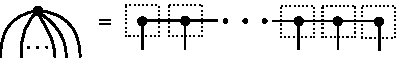
\includegraphics[width=0.75\textwidth]{fro-MPS1}
\end{center}
The {\sf GHZ}-state tensor is simply a order-$n$ {\sf COPY}-tensor.  Node
equivalence
implies that this tensor can be deformed into any network
geometry including a MPS comb-like structure (right).
\begin{center}
    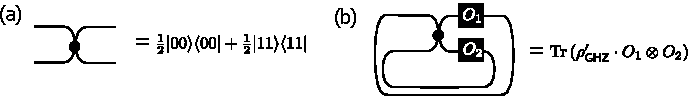
\includegraphics[width=\textwidth]{GHZreduced1}
    \label{fig:ReducedGHZ}
\end{center}
Reduced density operator.  Left (a) reduced density operator $\rho_{\sf GHZ}'$ found from applying the fusion law to a n-qubit {\sf GHZ}-state.  Right (b) the expectation value of observable $O_1\otimes O_2$ found from connecting the
observable and connecting the open legs (i.e.\ taking the trace).
\end{example}

\begin{myexercise}
Write down the matrix product state for the n-party GHZ  and n-party W-states. Let us define the two-point correlation as \begin{equation}
    C_{i,j}(\psi, A_i, A_j) =  \bra{\psi}A_i A_j \ket{\psi} - \bra{\psi}A_i  \ket{\psi}\bra{\psi}A_j \ket{\psi}
\end{equation}
Find $C(j\leq n):=C_{1,j}(\psi, X_1, X_j)$ for both GHZ- and W- where $X$ is the familiar Pauli matrix. Using Mathematica, make a publication quality plot for some fixed $n$ (e.g.~label everything and create a caption explaining the plot).  
\end{myexercise}

\begin{myexercise}[Basic properties of Boolean quantum states]
This exercise considers some elementary properties of Boolean quantum states.  
\begin{itemize}
 \item[(i)] Count the number of Boolean quantum states on n-qubits. Write truth tables for all two-input boolean functions and label appropriately those columns corresponding to \NOT, \AND, \XOR, \XNOR, \NAND, \NOR, and \OR.   
 \item[(ii)] Let $ \psi^2_{\7B} = c_0 \ket{00} + c_1\ket{01} + c_2 \ket{10} + c_3 \ket{11}$ represent a boolean quantum state, and hence $\forall i, c_i=0,1$.  Also let the output of all possible two-bit functions be 
 given by a truth vector $\textbf{c} = (c_0, c_1, c_2, c_3)$ and classify entangled vs non-entangled boolean states on two qubits.  
 \item[(iii)] Hence, using the result in (ii) or otherwise, show that the possible values of entanglement (using the quantity $K_1$ or $J_2$) is course grained and give the possible values.
\end{itemize}
\end{myexercise}



\begin{example}[valence-(0,3) tensor
factorization]\label{theorem:factorisation}
Every tensor in $\2A\otimes\2A\otimes\2A$ has a factorization as: (i) two valence-(1,0) tensors in $\2A$ (e.g.~the triangles); (ii) two valence-(2,1) \COPY-tensors; (iii) two unitary
morphisms of type $\2A\rightarrow\2A$ (white boxes).  This factorization is
given
diagrammatically as follows. 
\begin{center}
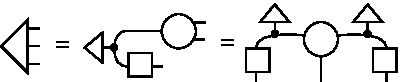
\includegraphics[width=8\xxxscale]{3-party-states}
%\epsfig{figure=pics/3-party-states,width=8cm}  
\end{center} 
\end{example}

\begin{myexercise}[MPS factorization of the \AND-state]
 Recall the MPS factorization of quantum states covered in lecture I.
Present an MPS factorization of the \AND-state
\be 
\psi_\wedge = \ket{000}+\ket{010}+\ket{100}+\ket{111}
\ee 
into five elementary tensors, as illustrated in Example
\ref{theorem:factorisation}.   Write this as a matrix product.  (Note: it
is acceptable to use a computer to calculate the SVD. Another method follows
from considering the eigenvalues of reduced density states.)
\end{myexercise}






\begin{myexercise}[The class of linear quantum states]
 We define the linear class of quantum states as quantum states of the form 
 \be 
 \psi_{\oplus L} = \sum c_1x_1\oplus c_2x_2\oplus ...\oplus c_nx_n \ket{x_1, x_2, ..., x_n}.
 \ee
 Here we will consider a 1D system.  What is the maximum possible $\chi$ (as defined in lecture I) in a partition in one of these states?  
\end{myexercise}


\begin{myexercise}[Correlations in polarity states (Optional)]
Here let us consider a state defined as 
\be 
\psi:=\sum (-1)^{f(\textbf x)}\ket{\textbf x},
\ee 
where the sum is over all $\textbf x$.  These states are often considered in quantum algorithm theory.  
Prove that $\psi$ is separable iff the function implements a linear function.  
\end{myexercise}





\begin{definition}[Boolean Density Operators]
 In general, a Boolean density matrix takes the following form.  
 \begin{equation} 
\begin{split}
\rho_{\7 B} & = \sum f(\x)f(\y)\ket{\x}\bra{\y} =\\
 & = \sum f(x_1, ..., x_k, ..., x_n)f(y_1, ..., y_k, ...., y_n) \ket{x_1, ..., x_k, ..., x_n}\bra{y_1, ..., y_k, ..., y_n}
\end{split}
\end{equation}
\end{definition}
\begin{myexercise}[The Boolean trace theorem]
Show that performing the partial trace over the kth subsystem of a Boolean density state results in 
 \begin{equation} 
\begin{split}
\text{Tr}_k \rho_{\7 B}  & = \delta_{x_k, y_k} \rho_{\7 B}= \\
 & =  \sum f(x_1, ...,x_k, ..., x_n)f(y_1, ..., x_k, ..., y_n) \ket{x_1, ..., x_n}\bra{y_1, ..., y_n}
\end{split}
\end{equation}
\end{myexercise}

\begin{myexercise}[Two-qubit entanglement]
To prepare for the next problem, here we will continue our study of two-qubit entanglement, by considering again the results in Lecture I.  
 \begin{itemize}
 \item[(i)] By considering a general quantum state
 \be 
 \alpha \ket{00} + \beta\ket{01}+\gamma\ket{10}+\delta\ket{11},
 \ee  
and by using wire bending duality, construct the induced matrix $M$. 
  \item[(ii)]  Show that $\text{Det}(M)$ vanishes identically for $\alpha = ac$, $\beta = ad$, $\gamma = bc$ and $\delta = bd$ with $a,b,c,d\in \7C$ and factor states of this type into a product of local states $\phi_1(a,b)\phi_2(c,d)$.  
  \item[(ii)] Using this result from (ii) or otherwise, show that $\text{Det}(M)$ vanishes iff the state giving rise to $M$ under wire duality takes the form $\phi_1(a,b)\phi_2(c,d)$.
 \end{itemize}
\end{myexercise}


\begin{myexercise}[Quantum \AND-tensors] 
With the contractions in Figure \ref{fig:andtensor} (a) and (b) in mind, consider instead the contraction with the state 
\be 
\alpha\ket{0} + \beta\ket{1},
\ee 
and hence, form an order-two tensor $T$ with components take values in $\alpha$ and $\beta$.  
\begin{itemize}
 \item[(i)] Write down the quantum state resulting from this contraction.  By bending a wire, write down the resulting two by two matrix, and label this $M(\alpha, \beta)$.  
 \item[(ii)] By considering the matrix determinant or otherwise, find the values 
 that $\alpha$ and $\beta$ must take for the state to be separable. 
 \item[(iii)] Consider now products of $M(\alpha, \beta)$.  Give a one sentence proof or disproof of the following statements:  The products of $M$ for (a) a magma (or groupoid); (b) a semigroup; (c) a monoid.  
 \item[(iv)] Are there values of $\alpha$ and $\beta$ that make a state local unitary equivalent to a bell-state? Are there values of $\alpha$ and $\beta$ that can break leg exchange symmetry in the state? 
\end{itemize}
\end{myexercise}  



\begin{myexercise}
~
\begin{itemize}
 \item[(i)] Write down the functions for a two-party bell state, a GHZ and a W state.  Use the trace theorem to provide analytical closed formula for the reduced density states found 
 from tracing over the last bit.  Expand this as a matrix and compare to the result obtained using standard methods.  
 \item[(ii)] Using standard properties of Boolean algebra, show that $\rho_{\7 B}^2 = \rho_{\7 B}$ and hence that $\rho_{\7 B}$ is a projector.
 \item[(iii)] Show that $U=\I -2\rho_{\7 B}$ is self-adjoint and unitary.  Give values for the matrix trace and determinant of $U$. 
 \item[(iv)] Show that $(1-\rho_{\7 B})$ and $(\rho_{\7 B})$ project onto eigenspaces of $U$ and relate the dimension of the subspaces to properties of the boolean function.   
\end{itemize}
\end{myexercise}







\begin{myexercise}
Define the Werner states acting on $\mathbb{C}_2\otimes \mathbb{C}_2$ as 
\begin{equation}
    \rho_r = r\ketbra{\phi^+}{\phi^+}+ \frac{1-r}{4}\I
\end{equation}
where $\sqrt{2}\ket{\phi^+}=\ket{00}+\ket{11}$ is the standard Bell state and $r$ takes only values in the real interval $[0,1]$. Find (i) the matrix trace of $\rho_r$ and (ii) the eigenvalues of $\rho_r$.  The concurrence is 
\begin{equation}
    C(\rho) = \text{max}\{\lambda_1 - \lambda_2 - \lambda_3 - \lambda_4, 0\}
\end{equation}
where $\lambda_1 \geq \lambda_2 \geq \lambda_3 \geq \lambda_4$
Using part (ii) or otherwise, find $C(\rho_r)$. 
\end{myexercise}



\begin{myexercise}[The Shannon effect --- Research]
For many fundamental functions one can design efficient circuits.
Is it possible to compute each function by an efficient circuit? In 
1949 Shannon proved that almost all functions are hard functions, optimal
circuits for almost all functions have exponential size and linear depth.
This was proved quite easily using a counting argument \cite{Weg87}. The number of circuits with small circuit size or
small depth grows much slower than the number of different Boolean
functions implying that almost all functions are hard. This means that
a random Boolean function is hard with very large probability.  
\begin{itemize}
 \item[(i)] The circuits we consider here don't have the same temporal structure enforced by classical gates.  In that regard, we have seen that the function for the \W-state can be realized using two \COPY-gates, one \AND, and one \OR.  
 \item[(ii)] With this observation in mind, what can we say about the Shannon effect in the present case?  
\end{itemize}
\end{myexercise}